\begin{activity} \label{A:2.3.1}
The position of a car driving along a straight road at time $t$ in minutes is given by the function $y = s(t)$ that is pictured in Figure~\ref{fig:2.3.A1}.  The car's position function has units measured in thousands of feet.  Remember that you worked with this function and sketched graphs of $y = v(t) = s'(t)$ and $y = v'(t)$ in Preview Activity~\ref{PA:2.3}.

\ba
\item On what intervals is the position function $y = s(t)$ increasing? decreasing?  Why?
\item On which intervals is the velocity function $y = v(t) = s'(t)$ increasing? decreasing? neither?  Why?
\item \emph{Acceleration} \index{acceleration} is defined to be the instantaneous rate of change of velocity, as the acceleration of an object measures the rate at which the velocity of the object is changing.  Say that the car's acceleration function is named $a(t)$.  How is $a(t)$ computed from $v(t)$?  How is $a(t)$ computed from $s(t)$?  Explain.
\item What can you say about $s''$ whenever $s'$ is increasing?  Why?
\item Using only the words \emph{increasing}, \emph{decreasing}, \emph{constant}, \emph{concave up}, \emph{concave down}, and \emph{linear}, complete the following sentences.  For the position function $s$ with velocity $v$ and acceleration $a$,
	\begin{itemize}
		\item on an interval where $v$ is positive, $s$ is \underline{\hspace{1.5in}}.
		\item on an interval where $v$ is negative, $s$ is \underline{\hspace{1.5in}}. 
		\item on an interval where $v$ is zero, $s$ is \underline{\hspace{1.5in}}.

		\item on an interval where $a$ is positive, $v$ is \underline{\hspace{1.5in}}.
		\item on an interval where $a$ is negative, $v$ is \underline{\hspace{1.5in}}. 
		\item on an interval where $a$ is zero, $v$ is \underline{\hspace{1.5in}}.

		\item on an interval where $a$ is positive, $s$ is \underline{\hspace{1.5in}}.
		\item on an interval where $a$ is negative, $s$ is \underline{\hspace{1.5in}}. 
		\item on an interval where $a$ is zero, $s$ is \underline{\hspace{1.5in}}.
	\end{itemize}
\ea

\end{activity}

\begin{marginfigure}[-18cm]
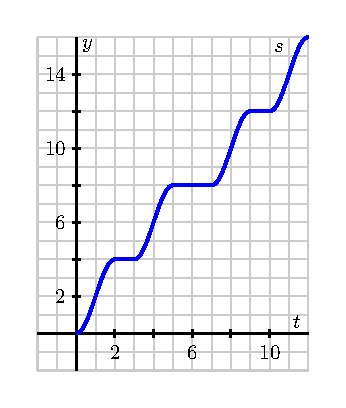
\includegraphics{figures/1_6_PA1.eps}
\caption{The graph of $y = s(t)$, the position of the car (measured in thousands of feet from its starting location) at time $t$ in minutes.} \label{fig:2.3.A1}
\end{marginfigure}


\begin{smallhint}
\ba
	\item Remember that a function is increasing on an interval if and only if its first derivative is positive on the interval.
	\item See (a).
	\item Remember that the first derivative of a function measures its instantaneous rate of change.
	\item Think about how $s''(t) = [s'(t)]'$.
	\item Be very careful with your letters:  $s$, $v$, and $a$. 
\ea
\end{smallhint}
\begin{bighint}
\ba
	\item Remember that a function is increasing on an interval if and only if its first derivative is positive on the interval and that $v(t) = s'(t)$.
	\item See (a), and note that $v'(t) = s''(t)$.
	\item Remember that the first derivative of a function measures its instantaneous rate of change, so $s''(t)$ measures the instantaneous rate of change of $v(t) = s'(t)$.
	\item Note that $s''(t) = [s'(t)]'$, so $s''(t)$ is the slope of the tangent line to $y = s'(t)$.
	\item Be very careful with your letters:  $s$, $v$, and $a$.  For instance, note that when acceleration is positive, velocity must be increasing.
\ea
\end{bighint}
\begin{activitySolution}
\ba
	\item The position function $y = s(t)$ increasing on the intervals $0<t<2$, $3<t<5$, $7<t<9$, and $10<t<12$, because at every point in such intervals, $s'(t)$ is positive.  For the provided function, $s(t)$ is never decreasing because its derivative is never negative.
	\item The velocity function $y = v(t)$ appears to be increasing on the intervals $0<t<1$, $3<t<4$, $7<t<8$, and $10<t<11$ because the curve $y = s(t)$ is concave up which corresponds to an increasing first derivative $y =s'(t)$.  Similarly, $y = v(t)$ appears to be decreasing on the intervals $1<t<2$, $4<t<5$, $8<t<9$, and $11<t<12$ because the curve $y = s(t)$ is concave down which corresponds to a decreasing first derivative $y =s'(t)$.  On the intervals $2<t<3$, $5<t<7$, and $9<t<10$, the curve $y = s(t)$ is constant, and thus linear, so neither concave up nor concave down.  
	\item Since $a(t)$ is the instantaneous rate of change of $v(t)$, $a(t) = v'(t)$.  And because $v(t) = s'(t)$, it follows that $a(t) = v'(t) = [s'(t)]' = s''(t)$, so acceleration is the second derivative of position. 
	\item Because $s''(t)$ is the first derivative of $s'(t)$, when $s'(t)$ is increasing, $s''(t)$ must be positive.
	\item For the position function $s(t)$ with velocity $v(t)$ and acceleration $a(t)$,
	\begin{itemize}
		\item on an interval where $v(t)$ is positive, $s(t)$ is \underline{increasing}.
		\item on an interval where $v(t)$ is negative, $s(t)$ is \underline{decreasing}. 
		\item on an interval where $v(t)$ is zero, $s(t)$ is \underline{constant}.

		\item on an interval where $a(t)$ is positive, $v(t)$ is \underline{increasing}.
		\item on an interval where $a(t)$ is negative, $v(t)$ is \underline{decreasing}. 
		\item on an interval where $a(t)$ is zero, $v(t)$ is \underline{constant}.

		\item on an interval where $a(t)$ is positive, $s(t)$ is \underline{concave up}.
		\item on an interval where $a(t)$ is negative, $s(t)$ is \underline{concave down}. 
		\item on an interval where $a(t)$ is zero, $s(t)$ is \underline{linear}.
	\end{itemize}
\ea
\end{activitySolution}
\aftera